\chapter{Machine learning and statistical methods}
\label{chapter:MLStat}

This chapter introduces the Machine Learning (ML) methods used in the two analysis described in this thesis to enhance the separation between the signal and the background, and also the statistical methods used to extract the signal.\\

\acrlong{MLlabel}~(\acrshort{MClabel}) is one of the core developing fields in computer science allowing the analysis of large and complex datasets, offering sophisticated techniques with a broad range of possible applications. Regarding high energy physics, the large amount of \acrshort{MClabel} simulations or data that is being recorded makes it a field well suited for the application of \acrshort{MLlabel} techniques. In this chapter, different multi-variate techniques used in this thesis are introduced, focusing on the classification methods used to improve signal and background separation.\\

In order to test the predictions of a given model, experimental data and \acrshort{MClabel} simulations are compared using statistical methods. This chapter describes the tools used to extract the production cross-section of a given signal and, in the absence of it, their upper limits.

\section{Machine Learning}

The deployment of \acrshort{MLlabel} methods is already reaching crucial tasks in \acrshort{ATLASlabel} such as online data recording with the implementation of neural networks in calorimetry FPGAs~\cite{Laatu:2022fni} or for particle reconstruction in trigger algorithms~\cite{ATLAS:2019uhp}, which result in more efficient triggers than previous ones.\\

For these cases, a neural network is trained to reduce the signal to background ratio, offering a high-level discriminating variable for a classification problem or providing a prediction of a certain quantity. These methods can outperform conventional algorithms as machine learning algorithms perform the classification or inference from multi-dimensional inputs, allowing the extraction of more complex correlations and functions, given enough data. In addition, \acrshort{MLlabel} methods scale easier than non-\acrshort{MLlabel} algorithms in terms of the size of the dataset and the amount of input variables, or features.\\

On the other hand, detector simulation is one of the most computational intensive tasks within \acrshort{ATLASlabel}, especially the calorimeter simulation, and solutions involving adversarial networks and auto-encoders are being studied to output faster and reliable output.\\

Regarding particle reconstruction and identification, examples of \acrshort{MLlabel} implementations can be found within the $\tau$ identification~\cite{ATLAS:2019uhp} or $b$-tagging algorithms~\cite{ATL-PHYS-PUB-2020-014}. In physics analyses, the use of \acrshort{MLlabel} is already standardised typically to reconstruct signal processes or to discriminate them from the background. In this case, the output is a high discriminating variable that can be used to define high-purity signal analysis regions, for example.\\

\acrshort{MLlabel} algorithms are not designed for a specific task. They consist in general models with hundreds of free parameters that are tuned using data. The process of optimising the internal parameters to correctly solve a specific problem is known as training the model. Depending on the available data, model and its application, several steps are needed to adequately perform and evaluate the training.\\

Generally, two types of \acrshort{MLlabel} algorithms can be distinguished: Supervised learning and Unsupervised learning models. The main difference is that the first requires fully labelled training data, namely each instance in the data is associated with a known output or target value (like the true mass of a particle). The labels allow the model to map the input features and output labels, to generalise the relationship and classify correctly unseen data. On the other hand, unsupervised learning models do not rely on labelled data and are then used to uncover hidden patterns or structures within the data itself (like detection of anomalies). In the context of this thesis, supervised approaches are used based on Neural Networks (NNs) and Boosted Decision Trees (BDTs).\\

The relationship between a machine learning model, its parameters and the input data can be formally expressed using  a statistical notation. The statistical model of a general \acrshort{MLlabel} algorithm is denoted as $\text{P}_\text{model}(\mathbf{x_i}; \boldsymbol{\theta})$ and is parameterised with a set of parameters $\boldsymbol{\theta}$ while $\mathbf{x_i}=(x_i^1,x_i^2,...,x_i^M)$ is the input feature set of a single input data point $i$ of the $\mathbf{X}=(\mathbf{x_1},\mathbf{x_2},...,\mathbf{x_N})$ dataset consisting of $N$ data points. $\text{P}_\text{data}$ is the true distribution that generates the data but is unknown. In the case of supervised learning, every data point has a label that categorises the event, $\mathbf{y}=(y_1,y_2,...,y_N)$.

\subsection{Performance}

The model performance is usually the decisive measure of a \acrshort{MLlabel} method and, depending on the objective, different metrics are used. In the context of the NN implemented in this thesis, the loss function and the Area Under the ROC Curve (AUC) are used. The loss function is the quantity optimised during the model training while the AUC is the quantity used to characterise the performance of the model.

\subsection{Loss function}

The loss function $E$ or cost function is optimised during the model training and represents the deviation of a model from the desired behaviour. To be suitable for minimisation, the function has to be differentiable. The choice of the loss function depends on the problem and requires optimisation. For supervised learning, the loss function depends on the true and predicted label values so the worse the prediction, the higher is the loss function.\\

It is standard to express the loss of the full dataset $\mathbf{X}$ as the average loss of the single data points $\mathbf{x_i}$,

\begin{equation}
    E(\mathbf{X},\boldsymbol{\theta})=\frac{1}{N}\sum_{i=1}^NE(y_i,\text{P}_\text{model}(\mathbf{X},\boldsymbol{\theta}))
\end{equation}

For regression problems the typical expression for a loss function is the mean square error~\cite{EncyclopediaofML}, 

\begin{equation}
    E_{MSE}(\mathbf{X},\boldsymbol{\theta}) = \frac{1}{N}\sum_{i=1}^N (y_i-\hat{y_i})^2,
\end{equation}

which is an average of the deviation from the true labels, with $\hat{y}_i$ is the predicted value. For binary classification, the so-called \textit{binary cross-entropy}~\cite{binarycross} is frequently used, 

\begin{equation}
    E_{BCE}(\mathbf{X},\boldsymbol{\theta}) = -\frac{1}{N}\sum_{i=1}^N y_i\cdot\log(\text{P}_\text{model}(\mathbf{X},\boldsymbol{\theta}))+(1-y_i)\cdot\log(1-\text{P}_\text{model}(\mathbf{X},\mathbf{\theta})),
\end{equation}

which is the negative log-likelihood of a Bernouilly distribution. A modified version is used in multi-classification problems. 

\subsection{Area Under the ROC Curve}

In the analyses presented in this thesis, the NN is trained to output a high-level variable with high separation between signal and background. Hence, the loss function is not the only important criteria as both the shape and the separation between the signal and background output distributions are essential to estimate the performance of the analyses. The quantity to evaluate the separation between signal and background for a given variable is the \textit{Area Under the ROC Curve} (AUC), and is the main decisive variable to choose a training in this thesis.\\

When considering two distinct variable distributions, one corresponding to a signal sample and the other to a background sample, the \textit{Receiver Operating Characteristic} (ROC) curve is defined as the signal efficiency against the background rejection, and displays the trade-off between signal efficiency and background rejection for a given classification threshold. The shape of the curve already provides a lot of the information regarding the overlap of the distributions, but the characteristic quantity is the integral of the curve, the AUC. Figure~\ref{ML:AUC} illustrates two example distributions with a different degree of overlap. The minimum value of the AUC is 0.5, when the overlap between the two distributions (discriminating variable) is total, while the maximum value is 1, when the distributions are totally separated. In the case of AUC=1, a cut in the discriminating variable is able to completely distinguish between signal and background.

\begin{figure}[htbp]
    \RawFloats
    \begin{center}
    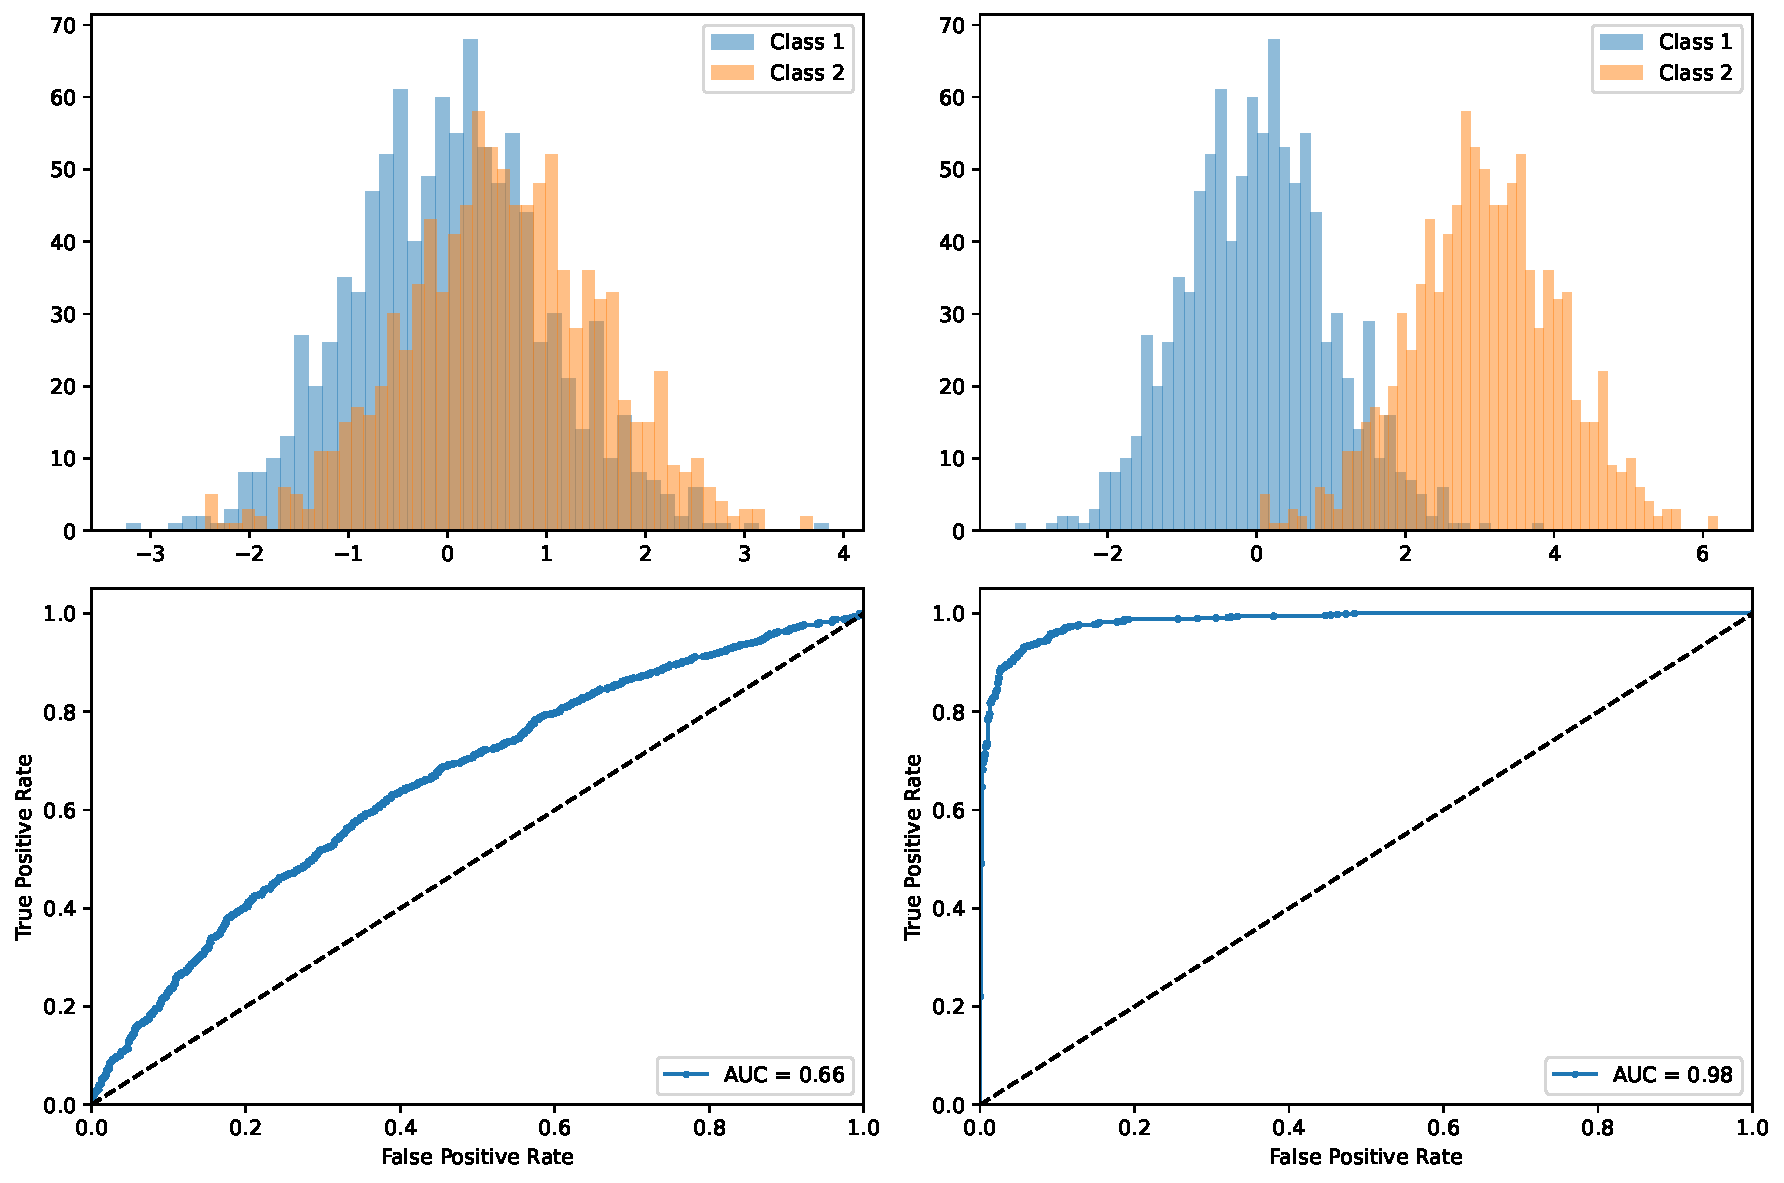
\includegraphics[width=0.75\textwidth]{ML/AUCexample.pdf}
    \caption{
        Comparison of two Gaussian distributions and their corresponding ROC curves to illustrate the behaviour of the ROC curve and the AUC.
    }
    \label{ML:AUC}
    \end{center}
\end{figure}

\subsection{Neural networks}
\label{ML:SectionNN}
Neural Networks (NNs) were introduced in the 1940s~\cite{McCulloch1943} but became feasible in the last decades as large computing power and GPUs are widely available. The concept of a NN consists of nodes (neurons) connected to each other via weights, and the most basic network is referred to as feed-forward NN.\\

An example is illustrated in Figure~\ref{ML:normalNN}, with in one input layer, one hidden layer and one output node. The result of the node has the form of a linear system $b+w\cdot x$, with bias $b$, weight $w$ and the input of the neuron $x$. More technically, the result of every node (except the input layer) is given by the sum of its inputs, the output of the different neurons connected to the given node multiplied by the weights $w_i$, which represent the connection. More generally, a bias $b_i$ is added to the sum and then used as input to an activation function $f_i$, which introduces non-linearity. The final output of the feed-forward NN in Figure~\ref{ML:normalNN} can be expressed as

\begin{figure}[htbp]
    \RawFloats
    \begin{center}
    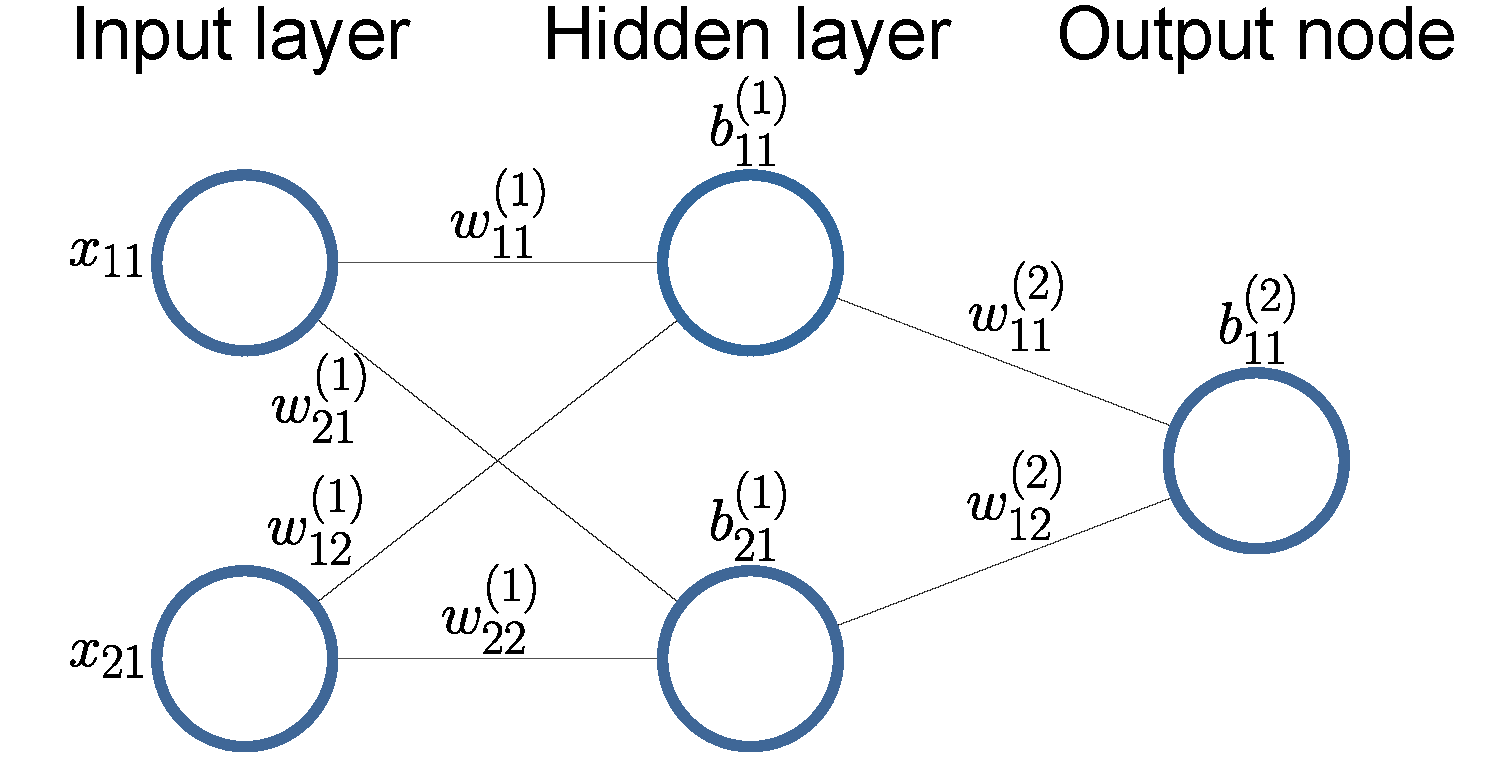
\includegraphics[width=0.75\textwidth]{ML/nnnormal.pdf}
    \caption{
        Fully connected feed-forward neural network with two input nodes, one hidden layer with two nodes and one output node.
    }
    \label{ML:normalNN}
    \end{center}
\end{figure}

\begin{equation}
    \text{P}_\text{model}(\mathbf{X},\boldsymbol{\theta}) = f_2(\mathbf{b_2}+\mathbf{W_2}f_1(\mathbf{b_1}+\mathbf{W_1}\mathbf{x})),
\end{equation}

with the inputs of a given data-point $\mathbf{x}$; the parameter set $\boldsymbol{\theta}$ including weight matrices $W_i$ and bias terms $b_i$. The index $i=1$ ($i=2$) denotes the hidden layer (output layer) and the two nodes in the hidden layer are assumed to use the same activation function. Fully expanding in matrix notation, the output of the NN can be written as

\begin{equation}
    \text{P}_\text{model}(\mathbf{X},\boldsymbol{\theta}) = f_2\left( \begin{bmatrix} b_{11}^{(2)} \end{bmatrix}+ \begin{bmatrix} w_{11}^{(2)} & w_{12}^{(2)}\end{bmatrix}f_1\left( \begin{bmatrix} b_{11}^{(1)} \\  
                                                            b_{21}^{(1)}  \end{bmatrix}+ \begin{bmatrix} 
    w_{11}^{(1)} & w_{12}^{(1)} \\ 
    w_{21}^{(1)} & w_{22}^{(1)}\end{bmatrix} \begin{bmatrix}
        x_{11}\\
        x_{21}
    \end{bmatrix} \right) \right)
\end{equation}

This simple example has nine free parameters $\boldsymbol{\theta}$ which are optimised during the training; more complex networks easily reach several ten-thousands of free parameters. Due to the non-linearity introduced by $f_i$, a NN can approximate any arbitrary function by giving the network enough freedom (amount of hidden layers and nodes). When a NN consists of multiple hidden layers, it is referred to as a deep learning~\cite{Goodfellow-et-al-2016} algorithm.\\

The main NN structure used in this thesis are feed-forward NNs, but there are a vast number of different architectures available developed for very different applications~\cite{livingreview}. Several software packages are available and accessible to the public,  mainly in Python, with popular examples as Pytorch~\cite{NEURIPS2019_9015}, Tensorflow~\cite{tensorflow2015-whitepaper} and Keras~\cite{chollet2015keras}. The main package used in this thesis is the latter, whose models are deployed in \acrshort{ATLASlabel} using the C++ based package lwtnn~\cite{lwtnn}.\\

The training of a NN is the process consisting on the optimisation of the free parameters $\boldsymbol{\theta}$ through a process called gradient descent, which iteratively adjusts the parameters by minimising the loss function. Apart from the free parameters, there are others that are manually set, called hyperparameters, and include for example the number of layers and nodes in the NN.\\

Batch training is a typical NN training procedure, where the minimisation of the loss function is done in steps with the training data divided into equally sized data fragments. At every step, the loss function is calculated using a segment of data and the internal parameters are updated. A full iteration over the entire dataset is referred to as an epoch. This batch training method makes the minimisation of the loss function faster. If the training would use the full dataset in one step it would end up profiling the very specifics of the training dataset, hence losing generalisation when evaluating other than the training data; this is called overtraining. The minimisation process could also stop in local minima thus not reaching the true performance.\\

For the batch training approach, the dataset is randomised and then split into an adequate dataset batch size to ensure that every batch is a correct representation of the dataset. Hence, the batch size is a hyperparameter of a NN training. If it is chosen too small, the minimisation is faster but the loss function may vary significantly at every step, and may lead to lower performance, as the model could end up being too general. On the other side, if the batch size is too large, the training could stop in a local minima.

\subsubsection{Optimiser}

After a first random initialisation of the free parameters $\boldsymbol{\theta}$, they are updated iteratively at each step of the training following the expression

\begin{equation}
    \theta' = \theta - l \nabla_\theta E(\theta;\mathbf{X}),
\end{equation}

where $l$ is the learning rate, also a hyperparameter, that tunes the rate of the update of the weights, and $\nabla_\theta E$ the gradient of the loss function with respect to a given free parameter. A large value of $l$ may prevent an optimal convergence of the loss function as the value might change the weights significantly between steps and may cause the minimisation process to behave erratically before reaching the minimum. On the other hand, an excessively low learning rate can slow the optimisation and cause the minimisation to stuck in a local minimum. Techniques that vary the learning rate or the batch size at every step can mitigate these extremes and gradually shift to a more precise minimisation of the loss function~\cite{LRBatchSize}. In this thesis, the Adam optimiser~\cite{Kingma2015AdamAM} which estimates of the first and second moment of the gradient, is used.

\subsubsection{Backpropagation}

For the gradient descend method, it is necessary to compute the gradient of the loss function with respect to all trainable parameters. However, calculating this gradient analytically for neural networks is unfeasible, as it involves nested gradients. Backpropagation~\cite{Rumelhart1986} is used to compute the gradient. It systematically calculates the nested gradients by applying the chain rule to traverse the entire network. To illustrate this, let us consider the chain rule for the loss function,

\begin{equation}
    \frac{\partial E}{\partial w_{ij}} = \sum_k \frac{\partial E}{\partial y_k} \frac{\partial y_k}{\partial w_{ij}},
\end{equation}

with $y_k$ being the output values of the neural network. The backpropagation algorithm calculates these partial derivatives efficiently through the reuse of intermediate results and considering parameter dependencies. 

\subsubsection{Activation Functions}

The introduction of activation functions $f(z)$ is essential to allow the neural networks to act as a non-linear function. Many candidates of activation functions exist, from simple step functions to monotonically increasing functions (as $\tanh$) or logistic functions (as the \textit{sigmoid} function). Although these activation functions are simple and manage to harmonise the inputs of a node, the resulting NN suffers from vanishing gradient issues which significantly slow down the training. The \textit{Rectified Linear Unit} ($\textsc{ReLU}$)~\cite{relu} activation function is widely used and is defined as

\begin{align}
    f_\textsc{ReLU}(z)= \begin{cases}
            0& \text{for}  z<0 \\
            z& \text{for}  z\geq0\\
            \end{cases}\qquad f'_\textsc{ReLU}(z)= \begin{cases}
                0& \text{for}  z<0 \\
                1& \text{for}  z\geq0\\
                \end{cases}.
\end{align}

This function is not affected by vanishing effects and the gradient is fast to compute, as the derivative function $f'(z)$ is very simple. Other popular activation functions are the Leaky $\textsc{ReLU}$~\cite{lrelu} and \textit{Softplus}~\cite{Maas2013RectifierNI}.\\

In general, the output nodes have different activation functions depending on the desired shape of the result. For classification problems, such as the neural networks used in this thesis, the output node can be evaluated with a sigmoid function, allowing the output to be interpreted as a probability,

\begin{equation}
    f_\text{sigmoid}(z)=\frac{1}{1+e^{-z}}.
\end{equation}

\subsubsection{Regularisation}

Besides the training performance, the ML model should be resilient to fluctuations in the training data or by the randomness of the training process itself. If performing the training with two equivalent datasets results in very different models and performance, it might be a strong indication of overfitting or other instabilities, which is difficult to study as a NN has many free parameters.\\

To protect the model's robustness, regularisation techniques are employed during the training. The most popular stochastic methods~\cite{JMLR:v15:srivastava14a,batchnorm,earlystop} are the introduction of dropout, batch normalisation or early stopping. The dropout method randomly removes an adjustable percentage (hyperparameter) of weights between neighbouring layers, thus avoiding strong correlations between neurons. Batch renormalisation consists on scaling the input of the layers while the early stopping method halts the training process after a given criterion to avoid overtraining. An early stopping method example could be to stop the training when the loss function calculated with the validation set does not improve after a certain amount of epochs. Another popular method, the L2 regularisation, consists in adding a term in the loss function that includes the sum of the squared weight values, thus penalising large weight values.\\

In this thesis, the dropout and early stopping methos are applied, while no big changes were seen when using other methods like the L2 regularisation method. The batch normalisation method is not applied, although an equivalent approach is applied to the input layer where the different input variables are scaled to have a mean value of 0 and a variance of 1. This avoids large differences in weights due to the difference of units between the input variables. One consideration is that distributions like \pT\ are not bounded like $\eta$ and outliers at the tail of the distributions can introduce instabilities to the model.

\subsubsection{Neural network parameterisation}

The analyses presented in this thesis use a NN technique referred to as parameterisation, usually applied to NN with signal or background events generated with different parameters. The parameterised NN~\cite{Baldi_2016} appears as a structure that simplifies training setups as it can replace various classifiers trained at individual values of a parameter. It is trained using the complete statistics reproduced with various values of the parameter, thus the training dataset is larger.\\

The NN has as input this parameter that distinguishes different classes of interest, like the training label set, a MC generator parameter or a source of uncertainty~\cite{Ghosh_2021}. Consequently, the response depends on the introduced parameters as depicted in Figure~\ref{ML:PNN}.\\

In the different searches presented in this thesis, the true mass of the new BSM particle is used as a parameter. As the parameter could be used by the NN to directly classify the events, the training should be set up appropriately. For signal events the parameter is set to correspond to the mass used to generate each signal sample, while for background events it is not well-defined and a random value is assigned to each event, reproducing the same mass distribution used for the signal events. This prevents the NN to directly use the parameter to perfectly classify the events, and the classification is optimised for each signal.

\begin{figure}[htbp]
    \RawFloats
    \begin{center}
    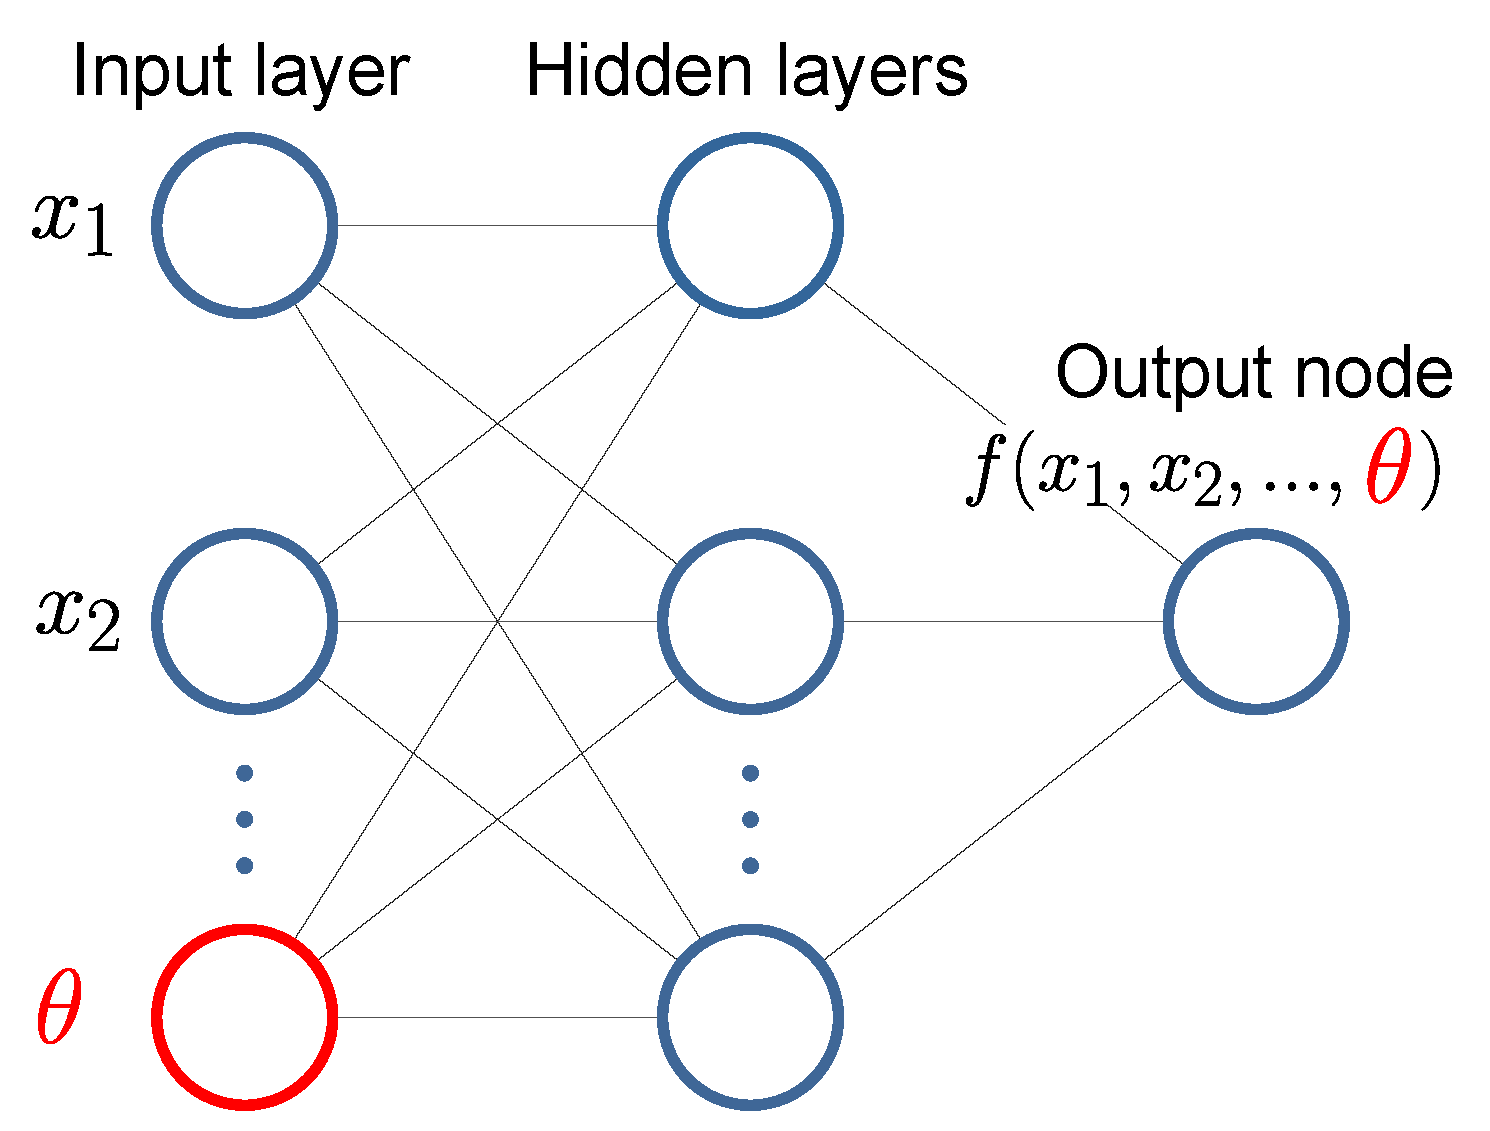
\includegraphics[width=0.75\textwidth]{ML/nntheta.pdf}
    \caption{
        Simple schematic of a fully connected feed-forward Neural network with input features $x_1, x_2,...$ as well as an input parameter $\theta$, such that the response $f$ depends on it.
    }
    \label{ML:PNN}
    \end{center}
\end{figure}

\subsection{Boosted decision trees}

Boosted decision trees (BDTs) were one of the most commonly used multivariate techniques in the last decade of high energy physics, before NNs became more accessible and popular. \\

The unit of a BDT is a decision tree, depicted in Figure~\ref{ML:BDT}. The structure is like a tree, as the name suggests, with branches connected via nodes. A cut on a specific input is made at each node, repeated until a stop criterion is met. The most common criteria are that the minimum events in a leaf is reached or that the maximum amount of cuts is reached (maximal tree depth). The decision tree alone is a weak learner and very sensitive to small changes in the training data, while an ensemble of weak learners leads to a powerful and robust model.\\


\begin{figure}[htbp]
    \RawFloats
    \begin{center}
    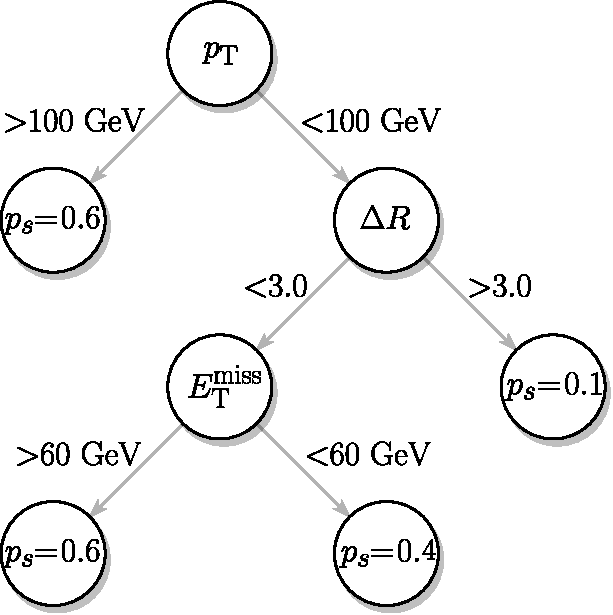
\includegraphics[width=0.75\textwidth]{ML/BDTtree.pdf}
    \caption{
        Schematic representation of a decision tree trained on a dataset composed of signal and background events with example training variables and cuts. The output of the tree is the probability that each event has of being generated by signal. Values above (below) 0.5 correspond to signal-like (background-like) events.
    }
    \label{ML:BDT}
    \end{center}
\end{figure}

Boosting is an ensemble technique for decision trees that combines their individual responses into a single discriminant

\begin{equation}
    \text{P}_{\text{model}} = \sum_{n=1}^N \alpha_n \text{P}_{\text{tree}}^{(n)}(\mathbf{x_i}),
\end{equation}

where $\text{P}_{\text{tree}}^{(n)}(\mathbf{x_i})$ denotes the statistical model of the decision tree $n$, $\mathbf{x_i}$ the input variables and $\alpha_n$ is a weight assigned to each tree's prediction. The boosting algorithm adjusts these weights to minimise the error in the prediction of the ensemble.\\

Different boosting methods are available, with the most popular ones for classification being Gradient Boosting (GradBoost) and Adaptive Boosting (AdaBoost)~\cite{FREUND1997119}. A GradBoost BDT~\cite{Chen_2016} involves training individual trees sequentially by computing the loss function, typically $E_{MSE}$, and adding the contribution of the next tree to the ensemble weighted such that the loss function minimised is

\begin{equation}
    E_n = E\left(\text{P}_{\text{model}}^{(n-1)}(\mathbf{x_i})+\alpha_n \text{P}_{\text{tree}}^{(n)}(\mathbf{x_i})\right).
\end{equation}

AdaBoost is a specific case where the weights of the events that are misclassified by a given tree are increased to have a greater impact in the loss function minimisation, hence enhancing learning in challenging phase spaces. Nevertheless, this can lead to a model sensitive to statistical deviations of the dataset or outlier events.\\

BDTs are implemented in \acrshort{ATLASlabel} software using ROOT~\cite{BRUN199781} via the TMVA~\cite{TMVA} package or more widely in python via scikit-learn~\cite{scikit-learn} or xgboost~\cite{Chen_2016}.

\subsection{Input data for training}

The selection of the dataset and its size depends on the problem that the \acrshort{MLlabel} is intending to solve. The datasets used in \acrshort{MLlabel} methods to discriminate between signal and background processes typically consist of simulated events. The choice of dataset and the number of inputs mostly depend on the problem's complexity and the desired performance, as more intricate scenarios require advanced algorithms with higher number of input variables and large datasets.\\

The input variables used in the \acrshort{MLlabel} trainings of this thesis can be categorised as low-level or high-level variables. The low-level variables are quantities of individual physics objects that have not been combined or designed to directly help the distinction between signal and background, like the kinematics of the objects of a collision event. High-level variables are referred to those obtained combining low-level variables and designed to offer discrimination, as reconstructed kinematics of a particular signal or the output of other classifiers, like $b$-tagging scores. Although high-level variables offer a lot of discrimination, a complete set of low-level variables has the necessary information to reach or even surpass the same level of discrimination, as correlations between variables can be exploited in advanced setups.\\

It is important to ensure an unbiased training process. For this purpose, the full dataset is split at least in two orthogonal samples, normally called training and validation datasets. The training dataset is used for the actual algorithm training, while the validation dataset is used to evaluate and monitor the final \acrshort{MLlabel} model. While a loss function is used to find the best set of parameters during the training, the performance on the validation set is evaluated in terms of sensitivity, selection efficiency, stability, and is used to fine-tune the model such as the choice of input variables or hyperparameters. Ideally, a third independent dataset (not used for training or for the choice of hyperparameters), referred to as testing set, is used to evaluate the final model. Some \acrshort{MLlabel} trainings performed in this thesis have not used a a testing set but no significant bias has been introduced, as the difference in performance between the validation and testing set is below statistical effects. In order to evaluate the full dataset, cross-validation (also named $k$-folding~\cite{EncyclopediaofML}) setups are used, where $k$ trainings are performed with the train/validation/test sets labelled accordingly, and every set is evaluated appropriately.\\

In this thesis as well as in typical \acrshort{ATLASlabel} analyses, every simulated event has an associated unique number not correlated with any physical variable. Hence, it is ideal to split the full dataset into the different sets using this number, like splitting the dataset into two with odd or even numbers. Another detail is that every simulated event has an event weight such that the sum for all events corresponds to the cross-section times luminosity and appropriately reproduces the expected kinematic distributions. In some cases the \acrshort{MClabel} weight is negative, which is almost exclusive to high energy physics datasets and, although the user-level \acrshort{MLlabel} tools accept event weights as input, their absolute value has to be used, as negative values are not properly defined in a \acrshort{MLlabel} training.

\section{Profile likelihood fit}
\label{sec:profilelikelihoodfit}

In order to test the compatibility between data and the \acrshort{MClabel} simulations, statistical methods in the context of hypothesis testing are used. The profile likelihood fit is a statistical tool used in this thesis to extract a measurement for the amount of the signal searched for in the analysis. When the presence of signal is not significant, upper limits are extracted based on the asymptotic formulation~\cite{Cowan_2011}. In this section, the profile likelihood fit method is presented with the necessary concepts in the context of a \acrshort{BSMlabel} search.
The technical implementation is provided by the RooStat framework~\cite{10.48550/arxiv.1009.1003}.\\

The fundamental idea behind hypothesis testing is to compare the agreement of the experimental data between two hypotheses and quantify which hypothesis can be discarded with a certain level of confidence. The two hypotheses to be compared are: the null-hypothesis $H_0$, corresponding to the~\acrshort{SMlabel} without new physics; and the alternative hypothesis $H_\mu$, which accounts for \acrshort{BSMlabel} interactions. The $\mu$ refers to the signal strength, commonly referred to as parameter of interest (POI), and is a normalisation factor for the sought signal,

\begin{equation}
    \mu = \frac{\sigma}{\sigma_{ref}}
\end{equation}

where $\sigma$ is arbitrary and $\sigma_{ref}$ is a reference value, typically a benchmark value from a theory or an expected sensitivity, like 1~pb. Hence, $H_\mu$ can be evaluated with a continuous spectrum of signal strengths and will approach the \acrshort{SMlabel} hypothesis ($H_0$) when $\mu\to0$.\\

Given a binned data distribution with $n_i$ events for a bin $i$, the expected value of $n_i$ can be expressed as

\begin{equation}
    E[n_i(\mu,\mathbf{b},\boldsymbol{\theta})] = \mu\cdot s_i(\boldsymbol{\theta}) + \sum_{k_{\alpha}\in\mathbf{k}}k_\alpha\cdot b_{\alpha,i}(\boldsymbol{\theta}),
\end{equation}

with $s_i$ being the predicted signal events and $b_{\alpha,i}$ the predicted background events of the process $\alpha$. The normalisation factor $k_\alpha$ affects the background process $\alpha$, analogous to $\mu$. Typically, $k_\alpha$ is introduced only for the most relevant backgrounds. The rest of the processes are normalised to their predicted cross-sections and the corresponding $k_\alpha$ is fixed to one. The nuisance parameters $\boldsymbol{\theta}$ are additional degrees of freedom which correspond to the systematic uncertainties acting both on the shape and normalisation of all processes. Their central value is defined to be zero and the deviation with respect to the original value is referred to as pull, where a deviation of $\pm$1 corresponds to a variation of one standard deviation.\\

The fit procedure allows the reduction of the impact of systematic uncertainties, especially by taking advantage of the highly populated background-dominated bins included in the fit. This requires a good understanding of the background and the systematic effects. To verify the improved background prediction, fits under the background-only hypothesis are performed, and differences between the data and the post-fit background prediction are checked using selections and physical variables other than the ones used in the fit.\\

The binned likelihood function is given as
\begin{equation}
    \mathscr{L}(\mu,\mathbf{k},\boldsymbol{\theta}) = \prod_i^N \frac{ (E[n_i(\mu,\mathbf{b},\boldsymbol{\theta})])^{n_i}}{n_i!}e^{E[n_i(\mu,\mathbf{b},\boldsymbol{\theta})]}\prod_{\theta_j\in\boldsymbol{\theta}}P(\theta_j)
\end{equation}

which corresponds to a product of Poisson probabilities and the penalty terms of all nuisance parameters for all $N$ bins. The form $P(\theta_j)$ are generally Gaussian distributions for each systematic uncertainty. Poisson distributions are used for the statistical uncertainty of each bin, and are introduced in the likelihood to penalise large deviations.\\

The optimal $\mu$, $\mathbf{k}$ and $\boldsymbol{\theta}$ are obtained from the fit to data that maximises the agreement between data and the prediction. The optimal test statistic to perform the fit is the likelihood ratio %https://link.springer.com/chapter/10.1007/978-1-4612-0919-5_5

\begin{equation}
    \lambda_\mu = \frac{\mathscr{L}(\mu, \hat{\hat{\mathbf{k}}},\hat{\hat{\boldsymbol{\theta}}})}{\mathscr{L}(\hat{\mu}, \hat{\mathbf{k}},\hat{\boldsymbol{\theta}})},
\end{equation}

with the single-hat parameters being those maximising the likelihood while $\hat{\hat{\mathbf{k}}},\hat{\hat{\boldsymbol{\theta}}}$ the parameters that maximise the likelihood for a given $\mu$. As the likelihoods are products of several terms smaller than one, a more stable test statistic is the negative log-likelihood

\begin{equation}
    q_\mu = -2\ln\lambda_\mu.
\end{equation}

For the purpose of setting upper limits on the signal production, some special cases are defined depending on $\mu$ and $\hat{\mu}$. If $\hat{\mu}$ is negative, i.e. the fitted signal has a negative normalisation, the modified test statistic assumes signal to be only positive: $\tilde{q}(\mu)=-2\ln\frac{\mathscr{L}(\mu, \hat{\hat{\mathbf{k}}},\hat{\hat{\boldsymbol{\theta}}})}{\mathscr{L}(0, \hat{\hat{\mathbf{k}}},\hat{\hat{\boldsymbol{\theta}}})}$, where the parameters in the denominator optimise the likelihood for $\mu=0$. Another exception is to set the modified test statistic to 0 for $\hat{\mu}>\mu$, as signal below the observed measurement is in complete agreement with the hypothesis.\\

The level of agreement between data and predictions for a given signal strength is quantified by computing the p-value $p_\mu$, which is the probability of the measured data being a deviation from the assumed $H_\mu$,

\begin{equation}
    p_\mu = \int_{q_{\mu,obs}}^\infty f(q_\mu|H_\mu)dq_\mu
\end{equation}

where $f(q_\mu|H_\mu)$ is the probability density function of $q_\mu$ under the assumption of $H_\mu$. The significance $Z=\Phi^{-1}(1-p_\mu)$ (being $\Phi$ the cumulative Gaussian distribution) is often preferred to quantify the level of disagreement in terms of the number of standard deviations. Typically, an alternative hypothesis is rejected at 1.64$\sigma$ ($p_\mu=0.05$) and the background-only at 5$\sigma$ ($p_0=2.87\cdot10^{-7}$).\\

Typically, searches are dedicated to very small signals that are difficult to separate from the background. Rejecting the null hypothesis at a fixed probability may result in excluding signals with low statistics not really searched for in the analysis~\cite{JUNK1999435}. The CL$_{s}$ method addresses this issue by defining

\begin{equation}
    \text{CL}_{s}=\frac{p_\mu}{1-p_0},
\end{equation}

where $p_0$ is the p-value for the null hypothesis, and $p_\mu$ is the p-value for the signal hypothesis. The ratio normalises the p-value to the confidence level of the background-only hypothesis such that the confidence level incorporates the information of both hypotheses and by construction is less prone to false discoveries or exclusions. The limits obtained using the CL$_s$ are conservative as when the measurement is not compatible with the null hypothesis, the denominator is larger and CL$_{s}$ decreases.

